\documentclass[12pt]{article}

\usepackage{graphicx}
\usepackage{paralist}
\usepackage{listings}
\usepackage{booktabs}
\usepackage{adjustbox}
\usepackage[font=small,labelfont=bf]{caption} 
\usepackage{float}
\restylefloat{table}

\oddsidemargin 0mm
\evensidemargin 0mm
\textwidth 160mm
\textheight 200mm

\pagestyle{plain}
\pagenumbering{arabic}

\newcounter{stepnum}

\title{SE2XB3 Requirements Specification: OptimizeU}
\author{SE2XB3 Group 8, L03}
\date{\today}

\begin{document}

\maketitle
\tableofcontents

\newpage
\section{Introduction}
The purpose of this document is to provide a requirements specification for
building an optimization system for Uber drivers to increase maximum uptime
for drivers and passengers alike.
\section{Domain}
\subsection{Application}
OptimizeU will have the following information:
\begin{itemize}
	\item \textbf{Uber pickups Dataset}:\\
	       Used to generate cluster information and pickup hotspots for
	       drivers to locate and pickup passengers
	\item \textbf{Graphical Interface}:\\
	       The output of algorithms performed on the dataset will be
	       displayed in a graphical user interface (GUI). Users will
	       navigate the GUI to obtain their desired information, such as 
	       optimized route for a particular time of the day.
\end{itemize} 
A more detailed functional and non-functional specification will be 
discussed later below.
\subsection{Stakeholders}
The stakeholders and their main relationships are listed below:
\begin{itemize}
	\item \textbf{Drivers}:\\
		These are the primary users of the application; They interact 
		directly with the program by obtaining location hotspots from
		certain times of days to get optimal travel routes and cluster
		visitations. 
	\item \textbf{Passengers}:\\
		Although passengers do not directly access the program, they
		are also considered a major stakeholder due to their relationship
		with drivers; passengers are the customers for the services that
		drivers provide.
\end{itemize}
\subsection{Goals, Expectations and Effects}
\begin{itemize}
	\item \textbf{Maximize driver's uptime and profits}:\\
		By smart optimization of driver's recommended locations and times
		to visit, more time will be spent on fetching passengers instead
		of finding for potential customers.
	\item \textbf{Improve passenger's wait times and safety}:\\
		Since more drivers are directed to passenger hotspots by usage
		of OptimizeU, passengers can enjoy minimized wait times and also
		street crime can be indirectly reduced as passengers spend less time
		waiting outside on streets.
\end{itemize}

\section{Functional Requirements}
The functional requirements will be documented using a use-case document (in
the form of a table), and a use-case diagram.

\begin{table}[H]
 \centering
  \begin{adjustbox}{max width=\textwidth}
  \begin{tabular}{*{2}{|l}|}
  \hline
  \textbf{Name:} & Get Optimized Routes\\
  \hline
  \textbf{Created By:} & SE2XB3 2018 Group 8\\
  \hline
  \textbf{Description:} & Uber driver instantiates the OptimizeU application\\
  \hline
  \textbf{Actors:} & Uber driver, OptimizeU Application\\
  \hline
  \textbf{Preconditions:} & 1. Uber driver has access to the OptimizeU application\\
  						  & 2. OptimizeU is fully functional\\
  						  & 3. Driver is in New York City area\\
  						  &	4. Security of the application or device is not compromised\\
  \hline
  \textbf{Postconditions:} & 1. Application retrieves and displays requested information successfully\\
                          & 2. Drivers get optimized routes from OptimizeU\\
  \hline
  \textbf{Flow:} & 1. Driver makes a request to the OptimizeU application\\
                 & 2. Application fetches dataset\\
                 & 4. Application uses dataset to process an optimized output\\
                 & 5. Application presents a GUI for the Driver to navigate\\
                 & 6. Driver uses GUI received to obtain the optimized driving route by hour of driving\\
  \hline
\end{tabular}
\end{adjustbox}
  \caption{Use Case Document in Table form}
  \label{usecase}
\end{table}
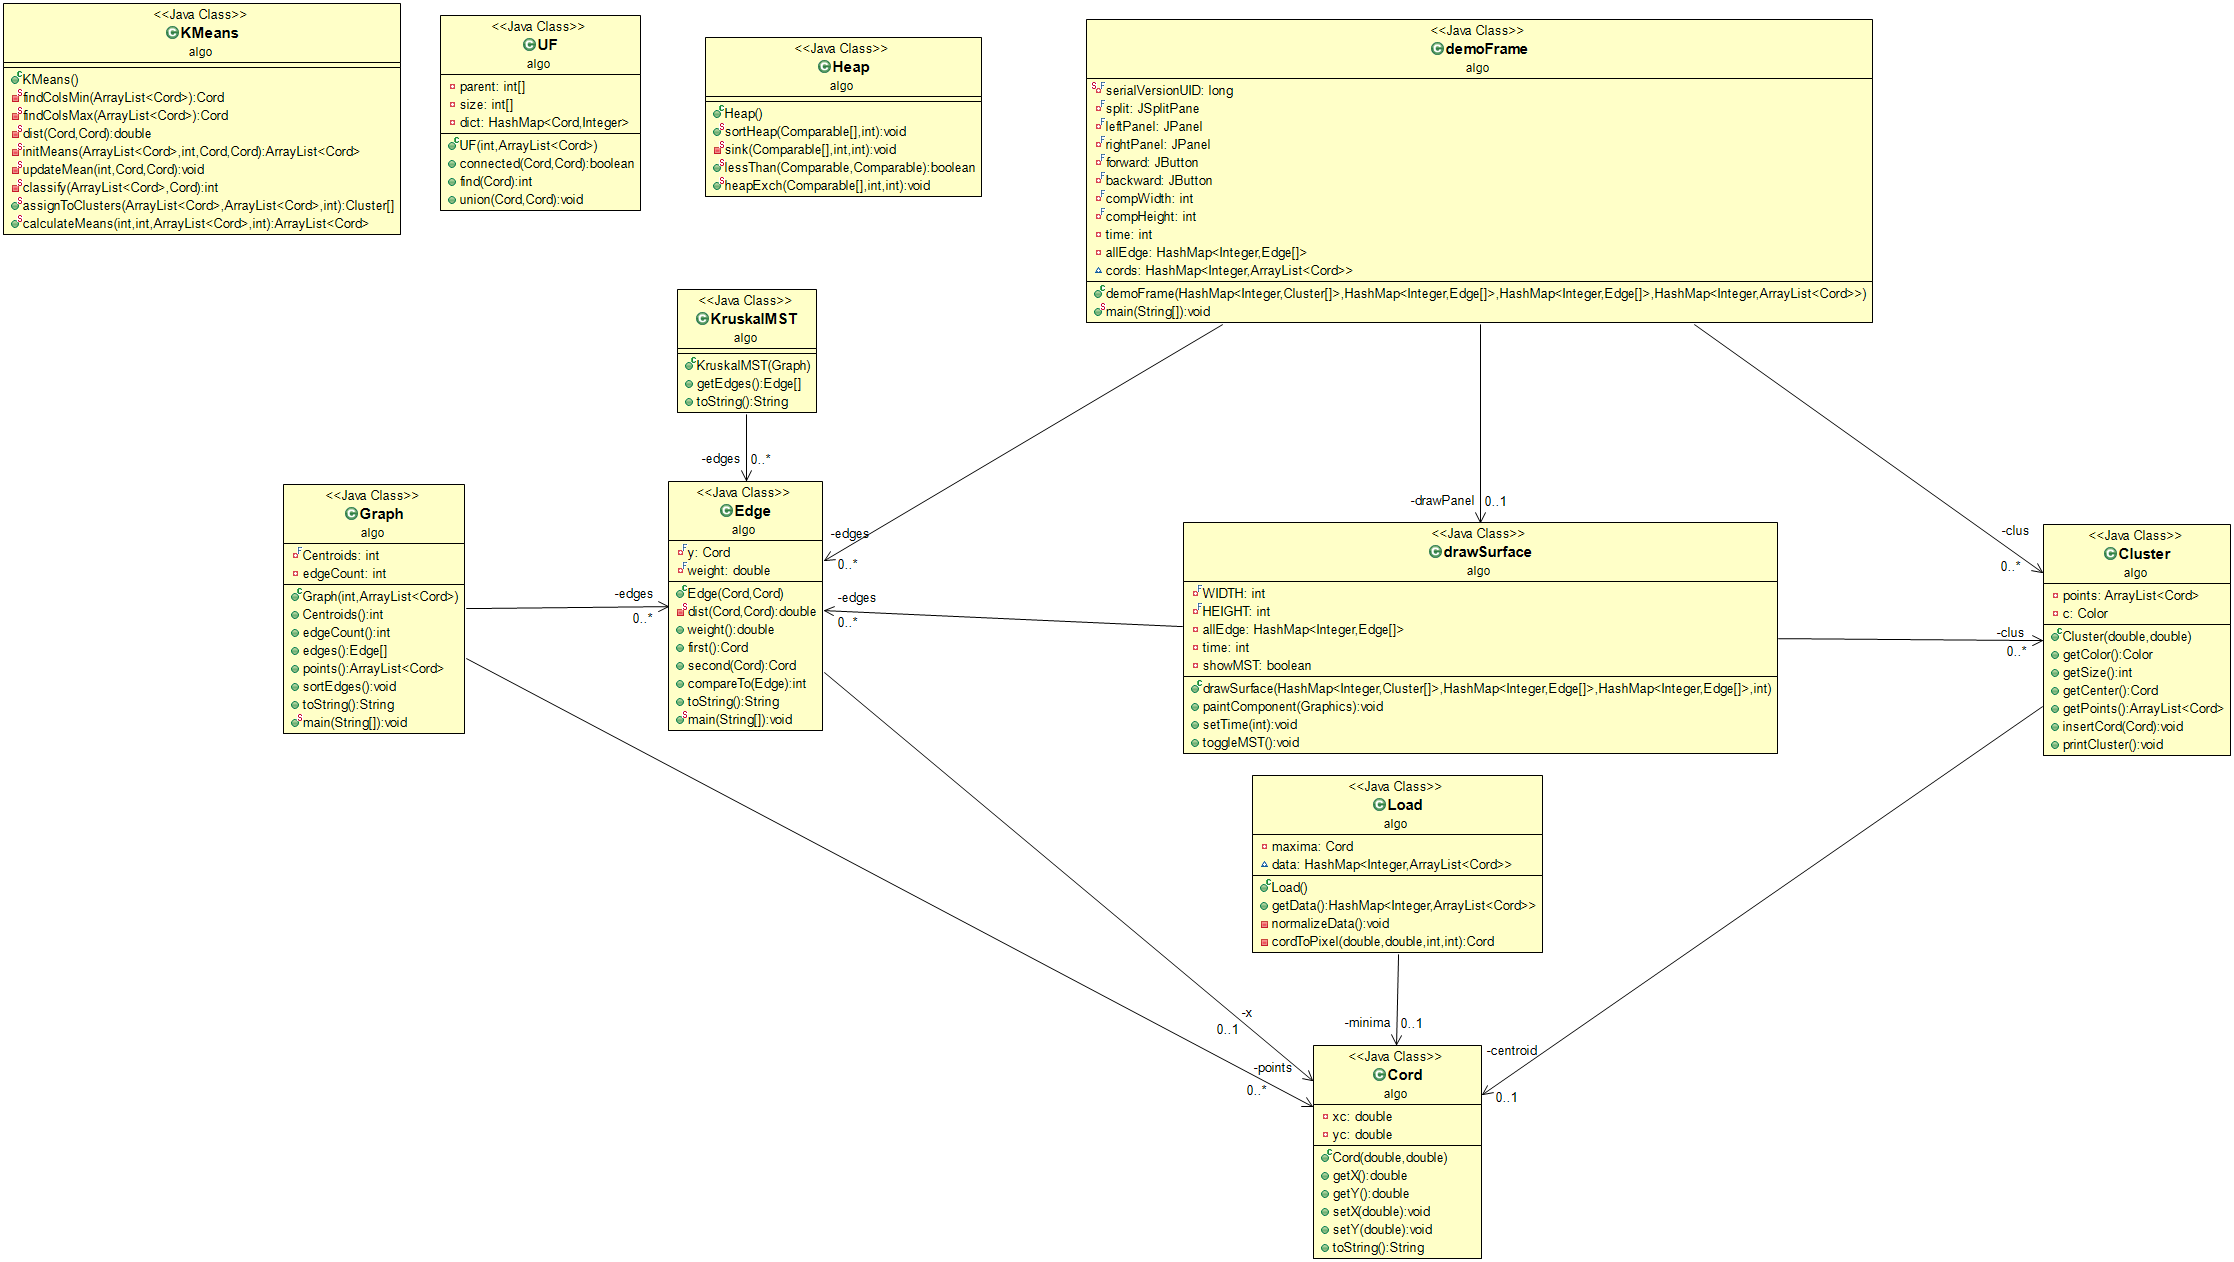
\includegraphics[width=100mm,scale=0.9]{UML.png}
\captionof{figure}{Uses Case Diagram}


\section{Non-Functional Requirements}
\subsection{Performance and Accuracy of Results}
OptimizeU should have the following capabilities:
\begin{itemize}
	\item \textbf{Adequate Application processing time:}\\
		Users should expect to get results within a reasonable time frame after submitting
		a request to the application. Depending on any external factors,
		users should expect a response within 3 seconds.
	\item \textbf{Consistent, accurate output}\\
		OptimizeU should consistently generate meaningful output for drivers to act on.
		An example being clustering that makes sense (e.g. a mega-cluster covering an 
		entire city wouldn't be of any use); or paths that are always minimal.
\end{itemize}
\subsection{Software Quality Attributes}
OptimizeU should possess the following software quality attributes:
\begin{itemize}
	\item \textbf{Reliability:}\\
		Generate optimized paths that are actually of use to the user. See the above
		section on consistency for an example.
	\item \textbf{Security:}\\
		As the dataset operates locally, care must be taken to ensure that the dataset
		is not compromised by any external factors, either intentionally or 
		unintentionally. Any compromise on the dataset will cause the entire application
		to fail or generate inaccurate output, which will affect the performance and 
		safety of its users.
	\item \textbf{Safety:}\\
		OptimizeU should ensure driver safety by providing appropriate route information.
		For example, routes should obey flow-of-traffic rules. This will probably
		be implemented as an extra feature, as this is not in scope of the project.
	\item \textbf{Portability Issues:}\\
		OptimizeU should be functional on relevant platforms. Since this is intended
		to complement the popular driving/on-hire app Uber, the intended platforms will
		be iOS and Android smartphones. Hence, it should be downloadable and usable 
		by users of both operating systems.
\end{itemize}
\section{Requirements on the Development and Maintenance Process}
\subsection{System test procedures}
The following system test must be carried out before the final product is ready:
\begin{itemize}
	\item \textbf{Algorithm/White box testing}\\
		Test critical algorithms rigorously to ensure that accurate information
		is always delivered to users.
	\item \textbf{GUI/Black box testing}\\
		Results that are being displayed must be tested to ensure output that is useful,
		consistent and beneficial to users.
\end{itemize}
\subsection{Priorities of Required Functions}
A list of required functions and their corresponding priorities are listed:
\begin{itemize}
	\item \textbf{K-Means}\\
		The clustering algorithm that is planned to be implemented. Must work on
		every occasion save on faulty or abnormal user input
	\item \textbf{Kruskal}\\
		The minimum-spanning tree path generation. Dependent on the correctness
		of k-medoids, but must also properly generate a MST on every clusters.
\end{itemize}
\subsection{Likely changes to System Maintenance Procedures}
\begin{itemize}
	\item Seperate tests may be carried out on similar algorithms (e.g. Prim vs Kruskal,
	K-Means vs K-Medoids etc.) if performance suffers. Change if necessary as well.
	\item Cluster generation: Since K-Means is strictly a heuristic, procedures can be 
	carried out to slightly modify clustering amounts to test the performance of each
	amount. An optimal amount can be selected, possibly for different input hours.
	\item Dataset updates: Since new data is constantly being created, OptimizeU may
	integrate additional datasets into the application to allow more accurate information
	to be available for users. Being able to sort output by month is the next step
	for OptimizeU.
\end{itemize}
\end{document}